\documentclass[dp]{FEIstyle}

% Author of the thesis
\FEIauthor{Bc. Maroš Kocúr}

% Evidence number
\FEIregNr{FEI-104376-111119}

% Title
\FEItitle{Autentifikácia emócií operátora na základe výrazu tváre}
\FEItitleEn{Operator's emotion authentication based on facial expression}

% Date
\FEIdate{14}{05}{2025}

% Keywords
\FEIkeywords{RGB kamera, neurónová sieť, ROS, autentifikácia, emócie, výrazy tváre}
\FEIkeywordsEn{RGB camera, neural network, ROS, authentication, emotions, facial expressions}

% Further details
\FEIstudyProgramme{Robotika a kybernetika}
\FEIstudyProgrammeEn{Robotics and Cybernetics}
\FEIstudyField{kybernetika}
\FEIstudyFieldEn{cybernetics}
\FEItrainingWorkplace{\a'Ustav robotiky a kybernetiky, FEI STU v Bratislave}
\FEItrainingWorkplaceEn{Institute of Robotics and Cybernetics, FEI STU in Bratislava}

% Supervisor
\FEIsupervisor{prof. Ing. Jarmila Pavlovičová, PhD.}

% Consultant
% -- if there is none, comment out the next line
\FEIconsultant{Ing. Michal Tölgyessy, PhD.}

% Glossaries -- terms and abbreviations.
% If you use automatic glossaries,
% uncomment the next line.
\FEIglossaries{includes/glossary}

% Bibliography database file
\bibliography{includes/bibliography.bib}

\usepackage[acronym]{glossaries}
\makeglossaries

\usepackage{tcolorbox}
\tcbuselibrary{listings,skins,breakable}

\newtcolorbox{codecell}[1][]{
    colback=gray!5!white,
    colframe=gray!75!black,
    fonttitle=\bfseries,
    title=Kód,
    #1
}

\newtcolorbox{outputcell}[1][]{
    colback=blue!5!white,
    colframe=blue!75!black,
    fonttitle=\bfseries,
    title=Výstup,
    #1
}

\begin{document}

%%%%%%%%%%%%%%%%%%
%%              %%
%% FRONT MATTER %%
%%              %%
%%%%%%%%%%%%%%%%%%
\frontmatter

\FEIpdfInfo
\FEIcover
\FEItitlePage
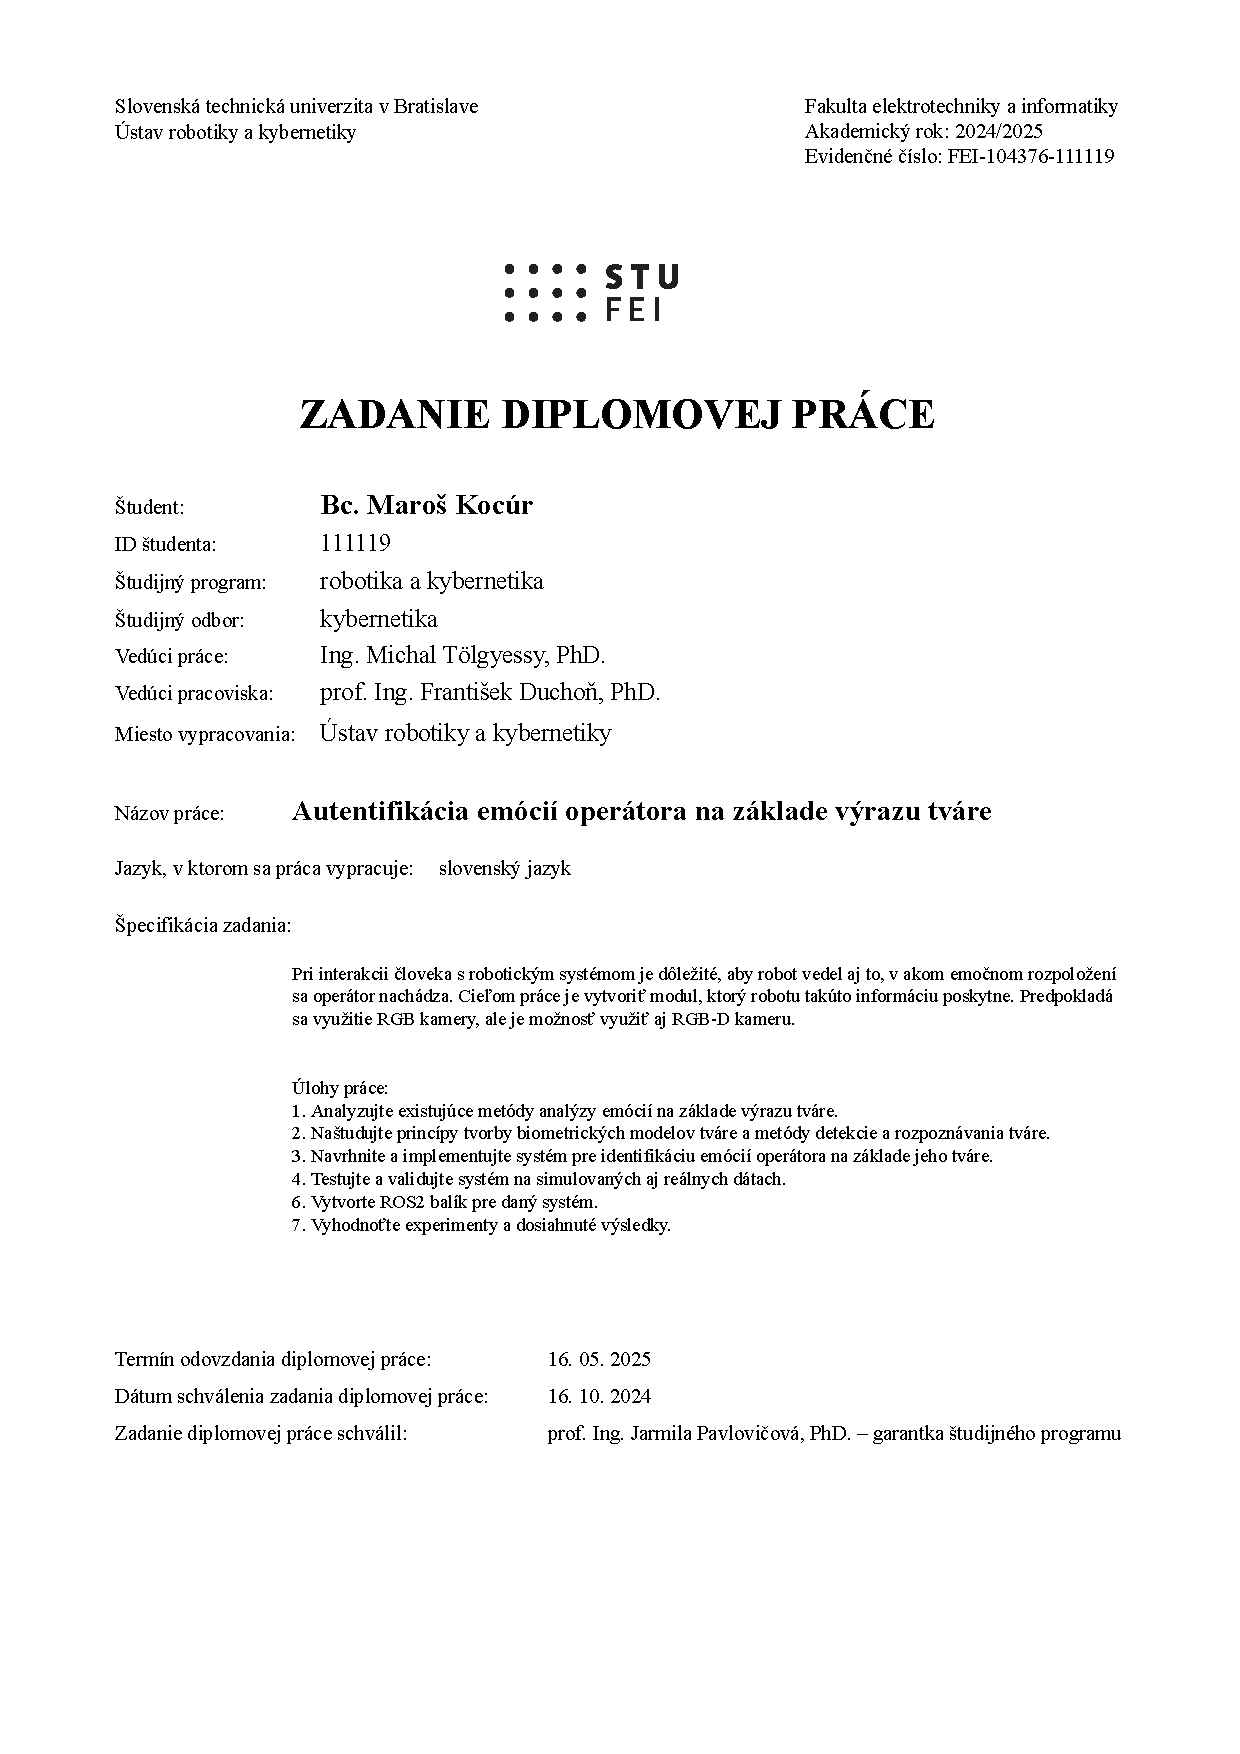
\includepdf[pages=-]{includes/assignment.pdf}
\FEIthanks{includes/thanks}
\FEIabstract{includes/abstract}
\FEIabstractEn{includes/abstractEN}
\FEIcontent
%\FEIlistOfFiguresAndTables

%% List of units and abbreviations
%%
%% Choose the method of typesetting the list of
%% units and abbreviations.
%% Uncomment only one of the two lines below!

%% METHOD 1:
%% ---------
%% Automatically generated and sorted list of
%% abbreviations with hyperlinks from the text.
%% Edit includes/glossary.tex.
%\FEIlistOfGlossaries
%% METHOD 2:
%% ---------
%% Manual list -- must be manually filled and sorted,
%% does not make hyperlinks from the text.
%% Edit includes/manual_glossary.tex.
% \FEImanualListOfGlossaries{includes/manual_glossary}
\FEIlistOfGlossaries
%% Lists of algorithms and listings
% \FEIlistOfAlgorithms
\FEIlistOfListings

%%%%%%%%%%%%%%%%%
%%             %%
%% MAIN MATTER %%
%%             %%
%%%%%%%%%%%%%%%%%
\mainmatter

\FEIintroduction{includes/introduction}
\FEIcore{includes/core}
\FEIconclusion{includes/conclusion}

%% Uncomment only if the document is writen in english
%\FEIresume{includes/resume}

%%%%%%%%%%%%%%%%%%
%%              %%
%% Bibliography %%
%%              %%
%%%%%%%%%%%%%%%%%%
\FEIbibliography
%% AI Declaration
\FEIaiDeclaration{includes/ai_declaration}

%%%%%%%%%%%%%%%%%%
%%              %%
%% BACK MATTER  %%
%%              %%
%%%%%%%%%%%%%%%%%%
\backmatter

%% Attachment A
\FEIappendix{Zdrojový kód pre rozpoznávanie emócií}{includes/attachmentA}

%% Attachment B
\FEIappendix{Zdrojový kód C++}{includes/attachmentB}

%% Attachment C
\FEIappendix{Zdrojový kód pre streamovanie snímok z kamier}{includes/attachmentC}

%% Attachement D
\FEIappendix{Zdrojový kód pre trenovanie modelu}{includes/attachmentD}

%% Attachement E
\FEIappendix{Zdrojový kód pre Docker}{includes/attachmentE}

%% Attachement E
\FEIappendix{Používateľský manuál}{includes/attachmentF}

\end{document}
